\documentclass{article}
\usepackage{graphicx} % Required for inserting images
\usepackage{amsmath}
\usepackage[colorlinks=true, pdfstartview=FitV, linkcolor=blue, citecolor=blue, urlcolor=blue]{hyperref}
\usepackage{babel}
\usepackage{har2nat}
\usepackage{float}
\usepackage[top=1.1in, bottom=1.1in, left=1.15in, right=1.15in]{geometry}
\usepackage{booktabs}
\usepackage{amssymb}
\usepackage{dsfont}
\DeclareMathOperator*{\argmax}{arg\,max}
\DeclareMathOperator*{\argmin}{arg\,min}

\title{Lista 2 - Organização Industrial}
\author{Arthur M. Rodrigues}
\date{October 2023}


\begin{document}

\maketitle

\section*{Questão 1}
Tome $M$ localidades indexadas por $m \in \{ 1, ..., M\}$, cada uma com uma usina potencial. O lucro de firma em $m$ é dado por:

\begin{equation*}
\Pi_m=
    \begin{cases}
        X_m\beta+\alpha I_{m-1}+\epsilon_m \text{, caso haja entrada}\\
        0 \text{, c. c.}
    \end{cases}
\end{equation*}

\subsection*{(a)}

Neste caso, cada firma consegue especificar e resolver o problema de outras usinas em todas as localidades, de modo que determinada firma potencial $m$ sabe a decisão de entrada nas localidades $1, ..., m - 1$ e portanto infere o valor de $I_{m-1}$ . Assim, cada firma avalia a condição de lucro positivo a partir de:

\begin{equation*}
\begin{aligned}
    m = 1 : \quad & X_1\beta+\epsilon_1 > 0 \therefore I_1 = \mathds{1}_{\{X_1\beta+\epsilon_1 > 0\}} \\
    m = 2 : \quad & X_2\beta+ \alpha I_1 + \epsilon_2 > 0 \therefore I_2 = \mathds{1}_{\{X_2\beta+ \alpha I_1 + \epsilon_m > 0\}} \\
    & \vdots \\
    m = M : \quad & X_M\beta+ \alpha I_{M-1} + \epsilon_M > 0
\end{aligned}
\end{equation*}

Desta forma, o sistema pode ser resolvido de forma recursiva. Conforme demonstrado em \citeasnoun{heckman78} , esta condição é necessária e suficiente para a existência de um equilíbrio único. Note que a unicidade do equilíbrio independe do sinal de $\alpha$: caso este seja negativo, há uma externalidade negativa da instalação de uma usina na localidade anterior, e caso positivo, esta externalidade é positiva. Entretanto, em ambos os casos o problema pode ser resolvido de forma recursiva. Sabendo a distribuição de $\epsilon$, podemos estimar o modelo a partir das probabilidades de entrada. Seja $F(\cdot)$ a c.d.f de $\epsilon$ e $P_m$ a probabilidade de entrada da firma $m$. Então temos:

\begin{equation*}
\begin{aligned}
        P_1 = & P(\epsilon_1 > - (X_1\beta)) = 1 - F(-X_1\beta) \\
    P_2 = & P(\epsilon_2 > -(X_2\beta+ \alpha I_1)) = 1 - F(-(X_2\beta+ \alpha I_1)) \\
    & \vdots \\
    P_M = & P(\epsilon_M > -(X_M\beta+ \alpha I_{M-1})) = 1 - F(-(X_M\beta+ \alpha I_{M-1}))
\end{aligned}
\end{equation*}

A partir dessas probabilidades, calculamos a verossimilhança amostral:

\begin{equation*}
    L(\theta) = \prod_{m=1}^{M} P_m ^{I_m} (1 - P_m)^{1 - I_m}
\end{equation*}

Então, podemos estimar o modelo a partir da maximização desta função de verossimilhança, o que é equivalente a um probit ordenado. Isto é:

\begin{equation*}
    \hat{\theta} = \argmax_\theta \log(L(\theta))
\end{equation*}

\subsection*{(b)}

Agora, as empresas não conseguem resolver o problema de todas as outras firmas, e a decisão de entrada se torna um problema estocástico em função do valor esperado do lucro em cada localidade $m$. O problema da firma 1 não é alterado:

\begin{equation*}
    m = 1 : X_1 \beta + \epsilon_1 > 0 \therefore P_1 = 1 - F(-X_1 \beta)
\end{equation*}

Entretanto, agora o valor de $P_{m-1}$, calculado a partir da distribuição de $\epsilon$, é necessário para para a resolução do problema da firma $m$ para $m = 2$ em diante:

\begin{equation*}
\begin{aligned}
        m = 2 : \quad & X_2 \beta + \alpha P_1 + \epsilon_2 > 0 \therefore P_2 = 1 - F(-(X_2 \beta + \alpha P_1)) \\
        m = 3 : \quad & X_3 \beta + \alpha P_2 + \epsilon_3 > 0 \therefore P_3 = 1 - F(-(X_3 \beta + \alpha P_2)) \\
        & \vdots \\
        m = M : \quad & X_M \beta + \alpha P_{M-1} + \epsilon_M > 0 \therefore P_M = 1 - F(-(X_M \beta + \alpha P_{M-1}))
\end{aligned} 
\end{equation*}

Note que, apesar da incerteza, o problema ainda pode ser resolvido de forma recursiva, de modo que o equilíbrio é único. Mais uma vez, essa constatação independe do valor de $\alpha$, que define se a externalidade da instalação de uma usina para a localidade rio abaixo é positiva ou negativa. A verossimilhança toma a forma:

\begin{equation*}
    L(\theta) = \prod_{m=1}^{M} P_m ^{I_m} (1 - P_m)^{1 - I_m}
\end{equation*}

E a estimação é feita a partir da maximização da verossimilhança amostral, de forma análoga ao item (a).

\subsection*{(c)}

Agora supomos que as firmas observam todo $\epsilon$ e que o lucro caso haja entrada toma a forma $\Pi_m=X_m\beta+\alpha I_{m-1}+\gamma I_{m+1}+\epsilon_m$, de modo que a construção de uma usina gera externalidade na localidade imediatamente acima e imediatamente abaixo do rio. Então, temos os seguintes casos dependendo dos valores de $\alpha$ e de $\gamma$.

\begin{itemize}
    \item $\alpha$ ou $\gamma = 0$
\end{itemize}


Nesse caso, se $\gamma = 0$ voltamos ao caso inicial do item (a) e temos unicidade no equilíbrio para qualquer valor de $\alpha$. Se $\alpha = 0$, temos um caso análogo com o problema recursivo sendo resolvido "de trás para frente", isto é, da localidade $m = M$ até $m = 1$:

\begin{equation*}
\begin{aligned}
 m = M : \quad & X_M\beta+\epsilon_M > 0 \therefore I_M = \mathds{1}_{\{X_M\beta+\epsilon_M > 0\}} \\
 m = M - 1 : \quad & X_{M-1}\beta+\gamma I_{M}+\epsilon_{M-1} \therefore I_{M-1} = \mathds{1}_{\{X_{M-1}\beta+ \gamma I_M + \epsilon_{M-1} > 0\}} \\
 & \vdots \\
 m = 1 : \quad &  X_{1}\beta+\gamma I_{2}+\epsilon_{1}
\end{aligned}
\end{equation*}

Assim, o problema ainda pode ser resolvido de forma recursiva e o equilíbrio é único para qualquer valor de $\gamma$.


\begin{itemize}
    \item $\alpha > 0$; $\gamma > 0$
\end{itemize}

Então, há externalidades positivas da construção de uma usina em $m$ nas suas localidades vizinhas $m+1$ e $m-1$. Não podemos garantir unicidade de equilíbrio nesse caso. Tome o seguinte contraexemplo com $M = 2$, $-X_1 \beta - \gamma < \epsilon_1 < -X_1 \beta$ e também $-X_2 \beta - \alpha < \epsilon_2 < -X_2 \beta$. Se ambas as firmas estiverem no mercado, não há incentivo para uma delas sair do mercado unilateralmente, enquanto se nenhuma estiver no mercado não há incentivo para uma delas entrar no mercado unilateralmente. Temos dois equilíbrios, um com ambas as firmas e outro com nenhuma.

\begin{itemize}
    \item $\alpha < 0$; $\gamma < 0$
\end{itemize}

Então, há externalidades negativas da construção de uma usina em $m$ nas suas localidades vizinhas $m+1$ e $m-1$. Também não podemos garantir unicidade no equilíbrio. Tome $M = 2$, $-X_1 \beta - \gamma > \epsilon_1 > -X_1 \beta$ e também $-X_2 \beta - \alpha > \epsilon_2 > -X_2 \beta$. Nesse caso, se nenhuma das firmas estiver no mercado, há incentivo para ambas entrarem, e se ambas estiverem há incentivo para ambas saírem. Entretanto, se qualquer uma das duas estiver sozinha, não há incentivo para a outra entrar e nem para ela sair. Temos dois equilíbrios, um com a firma de $m=1$ operando sozinha e um com a firma de $m=2$ operando sozinha.

\begin{itemize}
    \item $\alpha < 0$; $\gamma > 0$ (ou $\alpha > 0$; $\gamma < 0$)
\end{itemize}

Então, há externalidade positiva em um sentido e negativa em outro (ambos os casos são análogos). Nesse caso, é possível que o jogo não apresente equilíbrio em estratégias puras. Por exemplo, tome $M = 2$, com $\epsilon_1 \in [-X_1 \beta - \gamma, -X_1 \beta]$ e $\epsilon_2 \in [-X_2 \beta - \alpha, -X_2 \beta]$. Se $\alpha > 0$ e $\gamma < 0$, e a firma de $m=1$ está no mercado, a firma de $m = 2$ tem incentivos para entrar, mas caso a firma de $m=2$ entre, a firma de $m=1$ passa a ter incentivos para sair (ou o inverso se $\alpha < 0$ e $\gamma > 0$). Não há equilíbrios em estratégias puras.

\vspace{5mm}

Ou seja, tirando os casos particulares de $\alpha = 0$ ou $\gamma = 0$, temos possivelmente inexistência ou multiplicidade de equilíbrios, e não conseguimos escrever a função de verossimilhança e estimar o modelo diretamente como fizemos nos itens (a) e (b). Para realizar a estimação em caso de múltiplos equilíbrios, precisamos de uma estratégia que auxilie a escolha de um equilíbrio específico, como por exemplo definir uma firma como incumbente e transformar o problema em um jogo sequencial.

\section*{Questão 2}

Tome $n \in \{0, 1, ..., N\}$ firmas e considere os seguintes lucros para firmas que operam no mercado $i \in \{1, ..., M\}$:

\begin{equation*}
\begin{aligned}
    \Pi_i^E&=X_i\beta+h(n)-\Delta+\epsilon_i\\
    \Pi_i^I&=X_i\beta + h(n)+\epsilon_i\\
\end{aligned}
\end{equation*}

Em que o superescrito $E$ denota uma firma entrante e $I$ denota uma firma incumbente. Os lucros da firma fora do mercado são:

\begin{equation*}
\begin{aligned}
    \Pi_i^S&=-\Sigma\\
    \Pi_i&=0\\
\end{aligned}
\end{equation*}

Onde $S$ denota uma firma que operava no mercado e saiu dele.

\subsection*{(a)}

Temos uma base de dados com observações para cada localidade $i$ em um dado período $t$. Então, supondo que o número de empresas em $i$ é o valor de equilíbrio, a probabilidade de observar um mercado com $k \in \{1,...,N-1\}$ firmas na localidade $i$ é semelhante a de \citeasnoun{bresnahan1991entry} e dada por:

\begin{equation}
    P(k \text{ firmas}) = P(\Pi_i(n=k) \geq -\Sigma ; \Pi_i(n=k+1) < 0)
\end{equation}

Assim, não há incentivos para a $k$-ésima firma sair e nem para a entrada de uma nova firma $k+1$. Caso o número de firmas seja 0 ou $N$, temos as probabilidades:

\begin{equation*}
    \begin{aligned}
     P (0 \text{ firmas})&= P(\Pi_i(n=1) < 0)  \\
     P (N \text{ firmas})&= P(\Pi_i(n=N) \geq -\Sigma))
    \end{aligned}
\end{equation*}

Considerando $\epsilon \sim F$, podemos substituir as formas funcionais e obter:

\begin{equation*}
    \begin{aligned}
        P (0 \text{ firmas})&=1 - F(\Delta - h(1) - X_i\beta)\\
        P(k \text{ firmas}) &=F(-\Sigma - h(k) - X_i\beta) - F(\Delta - h(k+1) - X_i\beta)\\
        P(N \text{ firmas}) &= F(-\Sigma - h(N) - X_i\beta)
    \end{aligned}
\end{equation*}

Estas probabilidades nos permitem escrever a função de verossimilhança amostral e estimar os $\beta's$ por máxima verossimilhança com a forma funcional da verossimilhança amostral análoga a \citeasnoun{bresnahan1991entry}, que será explicitada na Questão 3. Entretanto, note que existem infinitas combinações possíveis os parâmetros $\Delta$, $\Sigma$ e do intercepto da função $h$ que correspondem à mesma probabilidade de entrada. Estes parâmetros não são unicamente determinados pelo processo gerador de dados que gera a amostra, de modo que não são unicamente identificados e a estimação nos dará no máximo um estimador agregado do intercepto que inclui $\Delta$, $\Sigma$, e o intercepto de $h$, enquanto podemos estimar o restante dos parâmetros de $h$ por métodos não paramétricos para lidar com a flexibilidade da função. Um problema similar aparece em \citeasnoun{bresnahan1991entry}, quando os autores argumentam que não distinguem entre custos fixos e afundados pois estes parâmetros não seriam unicamente identificados em uma \emph{cross-section}.

\subsection*{(b)}

Agora, temos dados para cada localidade $i$ nos períodos $t$ e $t+1$. Assim, podemos avaliar a variação de firmas nas localidades entre os períodos e escrever as probabilidades de forma similar a \citeasnoun{caballero2013efeitos}. Para cada localização $i$ na qual observamos $n$ firmas em $t=2$, temos os seguintes cenários:

\begin{itemize}
    \item Entraram firmas no mercado. Isso ocorre se o lucro para todas as firmas entrantes for positivo e se o lucro da "próxima" entrante potencial for negativo: $\pi_i^E(n)>0$, $\pi_i^E(n+1)<0$.
    \item Número de firmas no mercado se mantém. Isso ocorre quando o lucro da "próxima" entrante potencial for negativo, mas o lucro da $n$-ésima incumbente for melhor do que opção de saída: $\pi_i^E(n+1)<0$, $\pi_i^I(n)>Pi_i^S$.
    \item Saíram firmas do mercado. Isso ocorre caso o lucro da "última" firma a sair seja mais negativo que o custo de saída e o lucro da $n$-ésima incumbente não: $\Pi_i^I(n+1)<Pi_i^S$, $\Pi_i^I(n)>Pi_i^S$.
\end{itemize}

Portanto, assumindo $\epsilon \sim F$ e substituindo as formas funcionais, temos a seguinte probabilidade de observar um mercado com $k$ firmas em $t$ e $n$ firmas em $t+1$:

\begin{equation*}
    \begin{aligned}
P(n(t) = n, n(t+1) = k)=\left\{\begin{array}{cc}
F(\Delta - h(n + 1) - X_{it+1}\beta) - F(\Delta - h(n) - X_{it+1}\beta) & n > k \\
F(\Delta - h(n + 1) - X_{it+1}\beta) - F(-\Sigma - h(n) - X_{it+1}\beta) & n = k \\
F(-\Sigma - h(n + 1) - X_{it+1}\beta) - F(-\Sigma - h(n) - X_{it+1}\beta) & n < k
\end{array}\right
    \end{aligned}
\end{equation*}

Mais uma vez, os parâmetros $\Sigma$, $\Delta$ e da função $h$ não são unicamente identificados. \citeasnoun{caballero2013efeitos} lida com esse problema assumindo que o custo de saída é zero ($\Pi_i^S=0$) e estimando um parâmetro único para o intercepto. A estimação por máxima verossimilhança se daria a partir da maximização de:

\begin{equation*}
    \mathcal{L}(\theta)=\prod_{i=1}^M P(n(t+1)=n,n(t)=k)^{\mathds{1}_{[n_t=n,n_{t-1}=k]}}
\end{equation*}

\subsection*{(c)}

Agora, temos a mesma base de dados, mas supomos que as firmas são forward-looking. Este setup é parecido com o de \citeasnoun{bresnahan1994measuring}, e o valor esperado descontado do lucro da empresa que entra em $i$ em $t = \tau$ e sai em $t = T$ é dado por:

\begin{equation*}
    E\left[\sum_{t=\tau}^{T-1} \delta^{t-\tau}[X_{it}\beta + h(n_t) + \epsilon_{it}] - \Delta - \delta^{T}\Sigma \right]
\end{equation*}

Em que $\delta$ é o fator de desconto intertemporal. Mais uma vez, temos três casos possíveis:


\begin{itemize}
    \item Entraram firmas no mercado. Isso ocorre se o lucro esperado para todas as firmas entrantes for positivo e se o lucro da "próxima" entrante potencial for negativo: 
\begin{equation*}
\begin{aligned}
  X_{it+1}\beta + h(n(t+1)) + \epsilon_{it+1} + E\left[\sum_{t=t+2}^{T-1} \delta^{t-\tau}[X_{it}\beta + h(n(t)) + \epsilon_{it}] \right] \geq \Delta\\
    X_{it+1}\beta + h(n(t+1)+1) + \epsilon_{it+1} + E\left[\sum_{t=t+2}^{T-1} \delta^{t-\tau}[X_{it}\beta + h(n(t)) + \epsilon_{it}] \right] < \Delta
\end{aligned}
\end{equation*}
    
    \item Número de firmas no mercado se mantém. Isso ocorre quando o lucro da "próxima" entrante potencial for negativo, mas o lucro da $n$-ésima incumbente for melhor do que opção de saída: 

\begin{equation*}
\begin{aligned}
  X_{it+1}\beta + h(n(t+1)) + \epsilon_{it+1} + E\left[\sum_{t=t+2}^{T-1} \delta^{t-\tau}[X_{it}\beta + h(n(t)) + \epsilon_{it}] \right] \geq -\Sigma\\
    X_{it+1}\beta + h(n(t+1)+1) + \epsilon_{it+1} + E\left[\sum_{t=t+2}^{T-1} \delta^{t-\tau}[X_{it}\beta + h(n(t)) + \epsilon_{it}] \right] < \Delta
\end{aligned}
\end{equation*}
    
    $\pi_i^E(n+1)<0$, $\pi_i^I(n)>Pi_i^S$.
    \item Saíram firmas do mercado. Isso ocorre caso o lucro da "última" firma a sair seja mais negativo que o custo de saída e o lucro da $n$-ésima incumbente não:
\begin{equation*}
\begin{aligned}
    X_{it+1}\beta + h(n(t+1)) + \epsilon_{it+1} + E\left[\sum_{t=t+2}^{T-1} \delta^{t-\tau}[X_{it}\beta + h(n(t)) + \epsilon_{it}] \right] \geq -\Sigma\\
    X_{it+1}\beta + h(n(t+1)+1) + \epsilon_{it+1} + E\left[\sum_{t=t+2}^{T-1} \delta^{t-\tau}[X_{it}\beta + h(n(t)) + \epsilon_{it}] \right] < -\Sigma
\end{aligned}
\end{equation*}
    
\end{itemize}

Com os dados disponíveis, é impossível estimar este modelo, pois as probabilidaes dependem de dados de períodos futuros para os quais não temos informações.

\section*{Questão 3}

\subsection*{(a)}

Nesta questão, vamos verificar o comportamento dos thresholds populacionais de entrada $S_n$ e sua variância com o crescimento do número de firmas $n$ (nesse caso, revendedores de pneus). Para tal, vamos agrupar todos os municípios que possuem 5 ou mais firmas na categoria $n = 5$, de acordo com o paper original. Uma rápida análise de histogramas e densidades para diferentes $n$'s nos permite analisar como a distribuição de valores de população varia com o número de revendedores. Os resultados podem ser vistos na Figura \ref{fig 1}.

\begin{figure}[H]
    \centering
    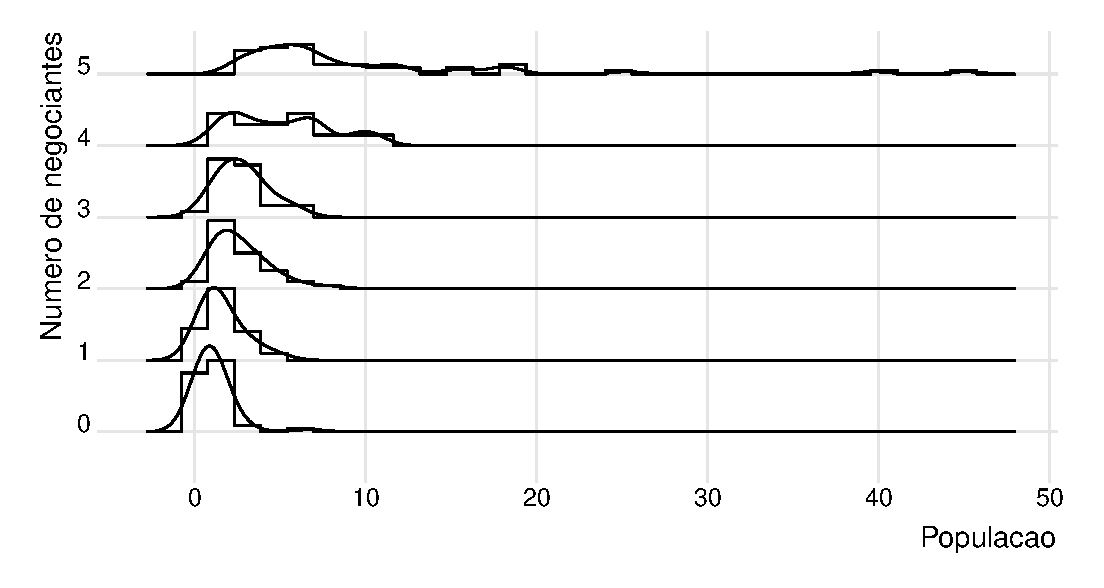
\includegraphics[width=\textwidth]{figs and tabs/histbres2.eps}
    \caption{Histogramas e Densidades - População por númer de Negociantes}
    \label{fig 1}
\end{figure}

Parece haver uma relação positiva entre número de empresas e população da cidade. Os histogramas das cidades com número maior de firmas também parece menos concentrado, com a implicação de que a variância dos thresholds aumenta com a população. O formato da distribuição para cidades com $n = 5$ parece distinto dos demais e contém alguns outliers com população bem superior, o que pode ser explicado pela decisão de agregar as cidades com 5 ou mais firmas e depõe contra esta decisão no paper original. Para checar se a intuição visual se confirma, podemos gerar uma tabela com a média e o desvio padrão da população condicionais ao número de vendedores, bem como o valor dos decis em cada subamostra.

\begin{table}[H]\centering
\begin{tabular}{r|r|r|r|r|r|r|r|r|r|r|r}
\hline
n & 0.1 & 0.2 &  0.3 &  0.4 &  0.5 &  0.6 &  0.7 &  0.8 &  0.9 & Média & $\sigma$\\
\hline\hline
0 & 0.39 & 0.50 & 0.63 & 0.74 & 0.92 & 1.04 & 1.19 & 1.31 & 1.68 & 1.09 & 1.04\\
\hline
1 & 0.65 & 0.77 & 0.91 & 1.05 & 1.17 & 1.35 & 1.67 & 2.44 & 3.40 & 1.62 & 1.16\\
\hline
2 & 1.03 & 1.43 & 1.64 & 1.79 & 2.22 & 2.69 & 3.16 & 3.79 & 4.47 & 2.64 & 1.60\\
\hline
3 & 1.20 & 1.73 & 1.90 & 2.11 & 2.59 & 3.07 & 3.36 & 3.78 & 4.84 & 2.80 & 1.40\\
\hline
4 & 1.99 & 2.23 & 2.82 & 3.93 & 4.65 & 5.92 & 6.82 & 7.00 & 9.10 & 5.08 & 2.96\\
\hline
5 & 3.36 & 4.21 & 5.28 & 5.86 & 6.51 & 7.56 & 9.75 & 12.07 & 18.14 & 9.71 & 9.01\\
\hline
\end{tabular}
\caption{Distribuição da População por Quantidade de Firmas}
\end{table}

De fato, cidades com mais firmas são em média mais populosas e apresentam dispersão maior na população. Entretanto, de modo geral, a previsão de que o aumento é mais que proporcional não se verifica no dado bruto. O crescimento populacional de duas para três firmas é especialmente baixo, de apenas 6\% na média e 16\% na mediana (e negativo no oitavo decil). O maior crescimento médio ocorre de 4 para 5 revendedores, mas é justamente a categoria agregada que originalmente continha observações com até 13 revendedores, tornando o resultado menos convincente.

\subsection*{(b)}

A última coluna da Tabela 4 de \citeasnoun{bresnahan1991entry} expõe o resultado de probits ordenados para as variáveis de número de vendedores de pneu na localidade. Para replicar esta tabela, vamos derivar a função de verossimilhança do paper original, no qual a função de lucro de uma empresa em dado mercado com $N$ empresas é dada por:

\begin{equation*}
    \Pi_N= \Bar{\Pi} + \epsilon = S(\mathbf{Y},\lambda)V_N(\mathbf{Z},\mathbf{W},\alpha,\beta)-F_N(\mathbf{W},\gamma)+\epsilon
\end{equation*}

Onde $S(\mathbf{Y}, \lambda) = tpop + \lambda_1 opop + \lambda_2 pgrw + \lambda_3 ngrw + \lambda_4 octy$ representa o número de consumidores, $V_{N}=\alpha_{1}+\mathbf{X} \beta-\sum_{n=2}^{N} \alpha_{n}$ é o lucro variável de break-even de $N$, e $F_{N}=\gamma_{1}+\gamma_{L} W_{L}+\sum_{n=2}^{N} \gamma_{n}$ é o custo fixo de $N$ ($W_L$ é um cost shifter da localidade, no caso a variável $landv$). Como não observamos diretamente $\Pi$, usamos os dados da presença ou não de firmas para derivar a verossimilhança. Substituindo as formas funcionais, temos:

\begin{equation*}
    \Bar{\Pi} = (tpop + \lambda_1 opop + \lambda_2 pgrw + \lambda_3 ngrw + \lambda_4 octy) * (\alpha_{1}+\mathbf{X} \beta-\sum_{n=2}^{N} \alpha_{n}) - \gamma_{1}+\gamma_{L} landv+\sum_{n=2}^{N} \gamma_{n}
\end{equation*}



Considerando $\epsilon \sim N(0,1)$, temos que as probabilidades são dadas por:

\begin{equation*}
\begin{aligned}
    P(0 \: \text{firmas}) &= P(\Pi_{1}<0) = 1-\Phi({\bar{\Pi}}_{1}) \\
    P(N \: \text{firmas}) &= P(\Pi_{N} \geq 0 \text { e } \Pi_{N+1}<0) = \Phi\left(\bar{\Pi}_{N}\right)-\Phi\left(\bar{\Pi}_{N+1}\right)\: \text{para}\: N = 1, 2, 3, 4 \\ 
    P(5 \: \text{firmas}) &= P(\Pi_{5} \geq 0) = \Phi(\bar{\Pi}_{5})
\end{aligned}
\end{equation*}

E portanto, a função de log-likelihood $\mathcal{L}$ para observações $i = 1, ..., I$ é:

\begin{equation*}
    \mathcal{L}=\sum\limits_{i=1}^I\left(\mathds{1}_{\{N_i=0\}}\log P\left(\Pi^i_1<0\right)+\mathds{1}_{\{N_i\geq5\}}\log P\left(\Pi^i_5\geq0\right)+\sum\limits_{j=1}^4 \mathds{1}_{\{N_i=j\}}\log P\left(\Pi^i_{N_i}\geq0\:\text{e}\:\Pi^i_{N_i+1}<0\right)\right)
\end{equation*}

Estimamos os parâmetros partir da maximização desta função de verossimilhança. Para replicar a Tabela 4 de \citeasnoun{bresnahan1991entry}, fixamos $\alpha_4 = \bar{\alpha_4} = 0$ e estimamos os demais 18 parâmetros livres, conforme metodologia do paper original. Como não há indicação dos palpites iniciais usados, definimos 0.01 como initial guess para todos os parâmetros.

\begin{table}[H]
    \centering
    \begin{tabular}{lrr}
\hline
 Parâmetro&Estimativa& Erro padrão assintótico\\
\hline
$\lambda_1$ &-0.53 & 0.40\\
$\lambda_2$ &2.25 & 0.97\\
$\lambda_3$ &0.34 & 0.61\\
$\lambda_4$ &0.23 & 0.41\\
$\alpha_1$ &0.86 & 0.46\\
$\alpha_2$ &0.03 & 0.12\\
$\alpha_3$ &0.15 & 0.09\\
$\alpha_5$ &0.08 & 0.05\\
$\beta_2$ &-0.49 & 0.63\\
$\beta_3$ &-0.03 & 0.03\\
$\beta_4$ &0.00 & 0.06\\
$\beta_7$ &-0.02 & 0.08\\
$\gamma_1$ &0.53 & 0.22\\
$\gamma_2$ &0.76 & 0.19\\
$\gamma_3$ &0.46 & 0.20\\
$\gamma_4$ &0.60 & 0.11\\
$\gamma_5$ &0.12 & 0.17\\
$\gamma_L$ &-0.74 & 0.40\\
Log-verossimilhança &-263.09&\\
\hline
\end{tabular}
    \caption{Replicação dos resultados de Bresnaham and Reiss (1991)}
    \label{repbresn}
\end{table}

A Tabela \ref{repbresn} apresenta parâmetros estimados iguais aos de \citeasnoun{bresnahan1991entry}. Entretanto, os valores dos erros padrão estimados são distintos. Isso ocorre pois a estimação do erro padrão assintótico é feita com a hessiana calculada numericamente a partir do problema de maximização especificado.

\subsection*{(c)}

Agora, estimaremos o modelo de forma idêntica ao item (a), mas sem fixar $\alpha_4 = 0$. Neste caso, estimamos 19 parâmetros livres, e mais uma vez utilizamos initial guesses de 0.01 para cada um deles. Podemos ver os resultados desta estimação na Tabela \ref{bresnalpha4}.

\begin{table}[H]
    \centering
\begin{tabular}{lrr}
\hline
 Parâmetro&Estimativa& Erro padrão assintótico\\
\hline
$\lambda_1$ &-0.46 & 0.43\\
$\lambda_2$ &2.29 & 1.00\\
$\lambda_3$ &0.48 & 0.67\\
$\lambda_4$ &0.20 & 0.44\\
$\alpha_1$ &0.82 & 0.46\\
$\alpha_2$ &0.04 & 0.11\\
$\alpha_3$ &0.17 & 0.09\\
$\alpha_4$ &-0.06 & 0.07\\
$\alpha_5$ &0.09 & 0.05\\
$\beta_2$ &-0.42 & 0.62\\
$\beta_3$ &-0.03 & 0.03\\
$\beta_4$ &0.01 & 0.06\\
$\beta_7$ &-0.02 & 0.08\\
$\gamma_1$&0.50 & 0.22\\
$\gamma_2$&0.74 & 0.18\\
$\gamma_3$&0.42 & 0.20\\
$\gamma_4$&0.76 & 0.24\\
$\gamma_5$&0.11 & 0.17\\
$\gamma_L$&-0.71 & 0.40\\
\hline
\end{tabular}
    \caption{Variante com $\alpha_4$ livre de Bresnaham and Reiss (1991)}
    \label{bresnalpha4}
\end{table}

De modo geral, os resultados são bem similares ao modelo restrito do item anterior (e do paper original). Particularmente, o coeficiente estimado para $\alpha_4$ não é estatisticamente significante. A justificativa do de \citeasnoun{bresnahan1991entry} para não estimar o parâmetro foi a imposição da restrição de $\alpha_N \geq 0\: \forall N$. Essa restrição parece razoável, já que espera-se $\overline{\Pi}_N \geq \overline{\Pi}_{N+1}$, isto é, que firmas que entram apenas em um threshold mais alto não tenham lucros maiores para o mesmo tamanho de mercado $S$. Parece uma escolha justificada, e o fato do modelo irrestrito não alterar muito os resultados depõe a favor do modelo.

\subsection*{(d)}

Agora, implementaremos um modelo baseado em \citeasnoun{seim2006empirical}, em que os $\varepsilon$'s (parte estocástica do lucro ou o \emph{tipo} das empresas) são considerados informação privada. Formalmente, um conjunto de $\mathcal{F}$ potenciais entrantes escolhem simultaneamente se entram em cada um dos mercados $m \in \{1, ..., M\}$ (neste caso, municípios). Como estamos supondo que os municípios possuem apenas um bairro, o vetor de localidades toma a forma $l \in \{0,1\}$, onde $l^f_m = 0$ representa a decisão de não entrar no mercado e $l^f_m = 1$ representa a de entrar. Assim, podemos omitir a notação do paper original de competição entre bands $b$ e cells $k$. Também omitiremos $l$ para as firmas entrantes e interpretaremos as características da única localidade de um mercado como características do mercado em si ($\mathbf{X}_m$ e $\varepsilon_{fm}$). Temos que o lucro da firma $f$ ao optar por entrar no mercado $m$ é dado por:

\begin{equation*}
        \Pi_{f}^m=\xi^m+\mathbf{X}_{m}\beta+\gamma \mathcal{E}^m +\varepsilon_{fm} = \bar{\Pi_f^m} + \epsilon_{fm}
\end{equation*}

Onde $\mathcal{E}^m$ é o número de entrantes no mercado $m$. Mas note que o $\varepsilon$ é informação privada, de modo que a decisão de entrada é de outras firmas não é conhecida, assim como o número de entrantes. Então, ao verificar o lucro esperado no mercado, as firmas avaliam o número de esperado de entrantes condicional a sua decisão de entrar:

\begin{equation*}
\begin{aligned}
        \mathbb{E}_f[\mathcal{E}^m | l_{f}^m = 1] &= (\mathcal{F}^m - 1)p_m + 1\\
        &\implies\\
        \mathbb{E}[\bar{\Pi^m_f}]= \xi^m+\mathbf{X}_{m}&\beta+\gamma*( (\mathcal{F}^m - 1)p_m + 1) +\varepsilon_{fm}
\end{aligned}
\end{equation*} 

Assumindo que as firmas são simétricas, podemos denotar $p_m$ como a probabilidade de uma entrante potencial escolher entrar no mercado $m$ condicional às informações que possui: $p_m = P(\text{entrada em } m | \xi^m, X_m, \theta_1)$, onde $\theta_1 = (\beta, \gamma) $. Ao assumir $\varepsilon \sim Gumbel(0)$, podemos calcular $p_m$ como:

\begin{equation}\label{pm}
    p_m = \frac{\exp(\bar{\mathbb{E}[\Pi_f^m}])}{1 + \exp(\mathbb{E}[\bar{\Pi_f^m})]}
\end{equation}

Como as firmas são simétricas e a probabilidade de entrada é igual para todas, também temos que observar:

\begin{equation}\label{E}
    \mathcal{E}=\mathcal{F}\cdot p_m \implies p_m = \frac{\mathcal{E}}{\mathcal{F}}
\end{equation}

De modo que podemos igualar \ref{pm} e \ref{E} e resolver para $\xi^m$, encontrando o valor de $\xi^m$ em cada mercado que garanta que o número de entrantes previsto no modelo sempre se verifique nos dados. Isso nos dá:

\begin{equation*}
    \xi^m = \log(\mathcal{E}) - \log(\mathcal{F}-\mathcal{E}) - (\xi^m+\mathbf{X}_{m}\beta+\gamma*( (\mathcal{F}^m - 1)p_m + 1))
\end{equation*}

Podemos tratar este valor de $\xi^m$ como o draw de uma distribuição normal $\xi^m \sim N(\mu,\sigma)$, em que $\mu$ e $\sigma$ são parâmetros que também serão estimados, com $\theta_2 = (\mu, \sigma)$. Como cada mercado $m$ é um jogo independente entre $\mathcal{F}^m$ firmas, temos que a verossimilhança amostral é dada por:

\begin{equation*}
    L(\theta_1,\theta_2)=\prod\limits_{m=1}^M\mathbf{p}_{\theta_1}(\mathbf{d}^m|\xi^m,\mathbf{X}^m,\mathcal{E}^m)g_{\theta_2}(\xi^m|\mathbf{X}^m,\mathcal{E}^m,\mathcal{F}^m)
\end{equation*}

Onde $\mathbf{d}^m$ é o vetor de escolhas de entrada das firmas potenciais $\mathcal{F}^m$ para um dado mercado $m$ e $g_{\theta_2}$ é a função de densidade da distribuição normal. Como nesse caso estamos lidando com uma decisão binária entre entrar e não entrar, a probabilidade $\mathbf{p}_{\theta_1}$ é dada simplesmente por $\mathbf{p}_{\theta_1}(\mathbf{d}^m|\xi^m,\mathbf{X}^m,\mathcal{E}^m) = p_m^{\mathcal{E}}(1-p_m)^{\mathcal{F} - \mathcal{E}}$. $g_{\theta_2}$. Assim, estimamos os parâmetros a partir da maximização do log desta verossimilhança, com as especificações de $\mathcal{F} = 50$ e $\mathcal{F}= 2 \mathcal{E}$. Para isto, descartamos as observações com 0 revendedores de pneu e consideramos o número original de revendedores por cidade (e não o restrito a no máximo 5, como em \citeasnoun{bresnahan1991entry}). Incialmente consideramos as mesmas variáveis de $X_m$ do que o modelo anterior, i.e. $eld$, $pinc$, $lnhdd$ e $ffrac$. Os initial guesses dos $\beta$'s foram os valoesr estimados na questão (c), e testamos $\gamma=-1$ e $\mu$ e $\sigma$ de uma normal padrão. Os resultados de $\mathcal{F} = 50$ e $\mathcal{F}= 2 \mathcal{E}$ podem ser avaliados nas Tabelas \ref{f50} e \ref{f2n}, respectivamente:

\begin{table}[H]
    \centering
\begin{tabular}{lrr}
\hline
 Parâmetro & Estimativa & Erro padrão assintótico\\
\hline
$eld (\beta_2)$ & -0.40 & 0.89\\
$pinc (\beta_3)$ & 0.07 & 0.04\\
$lnhdd (\beta_4)$ & -0.43 & 0.11\\
$ffrac (\beta_7)$ & -0.02 & 0.12\\
$\gamma$ & 1.06 & 0.09\\
$\mu$ &-0.88 & 1.01\\
$\sigma$ &0.50 & 0.03\\
\hline
\end{tabular}
    \caption{Modelo de Seim (2006) com $\mathcal{F}=50$}
    \label{f50}
\end{table}

\begin{table}[H]
    \centering
\begin{tabular}{lrr}
\hline
 Parâmetro & Estimativa & Erro padrão assintótico\\
\hline
$eld (\beta_2)$ &-1.47 & -\\
$pinc (\beta_3)$ & -0.01 & 0.01 \\
$lnhdd (\beta_4)$ & -0.06 & 0.01\\
$ffrac (\beta_7)$ & 0.12 & 0.02 \\
$\gamma$ & -0.02 & 0.01 \\
$\mu$ &0.76 & 0.11 \\
$\sigma$ & 0.09 & -\\
\hline
\end{tabular}
    \caption{Modelo de Seim (2006) com $\mathcal{F}=2\mathcal{E}$}
    \label{f2n}
\end{table}

Os dois modelos apresentam $\beta_3$ próximo de 0 e não estatisticamente significante, parecido com o modelo original de \citeasnoun{bresnahan1991entry}. Os parâmetros de $\beta_4$ e $\beta_7$ do modelo com $\mathcal{F}=50$ e $\mathcal{F}=2\mathcal{E}$ apresentam resultados estatisticamente significantes, o que não ocorria no modelo original. O resultado mais curioso se dá na estimação de $\gamma$ no modelo de $\mathcal{F}=50$, que é estatisticamente significante no sentido contrário ao esperado, indicando que um número maior de competidores em um mercado está associado a um lucro maior. Isso pode ocorrer porque, ao considerar apenas os $\beta$'s usados por \citeasnoun{bresnahan1991entry}, nós não estamos incluindo nenhuma característica populacional, que estava sendo medida pelos $\lambda$'s no modelo original, e o $\gamma$ pode estar captando um efeito de cidades maiores com mercados mais desenvolvidos serem mais lucrativas e atraírem mais competidores. Futuramente, convém rodar especificações com combinações diferentes de variáveis e ver se o sinal e magnitude estimados se mantém. Um problema adicional da estimação do modelo com $\mathcal{F}=2\mathcal{E}$ é que a estimativa da variância assintótica a partir da hessiana calculada numericamente para $\sigma$ e $\beta_2$ retorna valores negativos, de modo que não é possível reportar o erro padrão para estes estimadores. Esse fenômeno pode ser explicado por erros numéricos na computação da hessiana.

\bibliographystyle{ecta}
\bibliography{references}

\end{document}
